\section{Lecture 15 - 10/12/2022}

\subsection{Jump Theorem for Cauchy Integrals}
Let $\gamma \in PC^1$ with image $\Gamma := \gamma([a, b]) \subset \Cbb$, and let $f(z)$ be a continuous function on $\Gamma$.

\begin{definition}
The \textbf{Cauchy Integral} of $f(z)$ along $\gamma$ is the function
\[F(\xi) \coloneqq \frac{1}{2\pi i} \int_\gamma \frac{f(z)}{z - \xi} dz, \forall \xi \in \Cbb \setminus \Gamma\]
Note that as we take $\xi$ to infinity, $F(\xi) = 0$. Furthermore, $F(\xi)$ is analytic on $\Cbb \setminus \Gamma$ since it could be represented in power series by geometric expansion.
\end{definition}

\begin{example}
If $\gamma$ is a closed loop and $f(z)$ is identically $1$, then the Cauchy integral of $f(z)$ around $\gamma$ is exactly the winding number $F(\xi) = w(\gamma, \xi)$ of $\gamma$ around $\xi$, which is either $1$ if the point is inside or $0$ if the point is outside.
\end{example}

\begin{theorem}[Plemelj-Sokhotsky Theorem]
Let $\gamma$ be a simple $C^1$-closed curve, and $f \in C^1_\Cbb(\gamma)$. Note that the Cauchy Integral $F(z) = \frac{1}{2\pi i} \int_\gamma \frac{f(\xi)}{\xi - z} d\xi$ is undefined for any $z \in \gamma$ but is defined on the interior and exterior of the curve, which we will denote by $F_+$ for interior and $F_-$ for exterior respectively.\\\\
Now take $z_0$, we have that
\[F_{\pm}(z_0) = \frac{1}{2\pi i} p.v. \int_\gamma \frac{f(\xi)}{\xi - z_0} d\xi \pm \frac{1}{2} f(z_0)\]
\end{theorem}

\begin{proof}
    First we rewrite
    \[\int_\gamma \frac{f(\xi)}{\xi - z} d\xi = \int_\gamma \frac{f(\xi) - f(z)}{\xi - z} d\xi + \int_\gamma \frac{f(z)}{\xi - z} d\xi\ (*)\]
    Now let $\delta > 0$ be chosen appropriately and consider the disk $D_{z_0, \delta}$ such that the domain of where $f$ is homolomorphic contains the closure of the disk (recall $f$ being holomorphic on compact $\gamma$ means there exists some open set containing $\gamma$ that $f$ is holomorphic on). Then since $\nabla f$ is a continuous function on compact $\overline{D_{z_0, \delta}}$, $|\nabla f|$ is bounded on the the disk.\\\\
    Thus, by Dominated Convergence Theorem, as we take the limit as $z \to z_0$:
    \[\lim_{z \to z_0} \int_\gamma \frac{f(\xi) - f(z)}{\xi - z} d\xi = \int_\gamma \lim_{z \to z_0} \frac{f(\xi) - f(z)}{\xi - z} d\xi = p.v. \int_\gamma \frac{f(\xi)}{\xi - z_0} d\xi - p.v. \int_\gamma \frac{f(z_0)}{\xi - z_0} d\xi\]
    There are two more things that we want to check:
    \begin{itemize}
        \item The principal value of $\int_\gamma \frac{1}{\xi - z_0} d\xi$ exists
        \item The following limit is true \[\lim_{z \to z_0, \text{interior}} \int_\gamma \frac{1}{\xi - z} d\xi = p.v. \int_\gamma \frac{d\xi}{\xi - z_0} + \pi i\]
    \end{itemize}
    Then it follows from the limit and our prior computation that:
    \begin{align*}
        F_+(z_0) &= \frac{1}{2\pi i} \cdot [p.v. \int_\gamma \frac{f(\xi)}{\xi - z_0} d\xi  - p.v. \int_\gamma \frac{f(z_0)}{\xi - z_0} d\xi] + \frac{1}{2\pi i} \cdot [p.v. \int_\gamma \frac{f(z_0) d\xi}{\xi - z_0} + f(z_0) \pi i]\\
        &= \frac{1}{2\pi i} p.v. \int_\gamma \frac{f(\xi)}{\xi - z_0} d\xi + \frac{1}{2} f(z_0) \tag*{We can cancel the principal values because they exist}
    \end{align*}
    A similar argument will also prove the case for $F_{-}(z_0)$. It then remains for us to prove the two claims:
    \begin{enumerate}
        \item For existence, let $\gamma_\delta \coloneqq \gamma \cap D_{z_0, \delta}$ and let $\gamma^\delta \coloneqq \gamma \setminus \gamma_\delta$. In other words, the latter is $\gamma$ with its path in the disk removed, then we have that
        \[\int_\gamma \frac{d\xi}{\xi - z} = \int_{\gamma_\delta} \frac{d\xi}{\xi - z} + \int_{\gamma^\delta} \frac{d\xi}{\xi - z}\]
        Now consider the following contour:
        \[\fbox{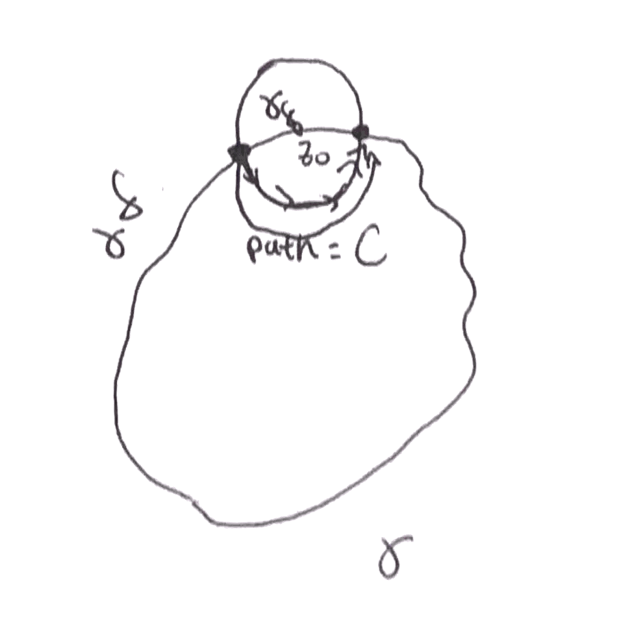
\includegraphics[width=.4\textwidth]{Figures/gamma-delta.png}}\]
        Then by Cauchy's Theorem
        \[\int_{\gamma_\delta} - \int_C = 0\]
        Hence we have that
        \[\int_\gamma \frac{d\xi}{\xi - z} = \int_{C} \frac{d\xi}{\xi - z} + \int_{\gamma^\delta} \frac{d\xi}{\xi - z} \]
        Then as we take the limit and exchange it with the integral using uniform convergence:
        \[\lim_{z \to z_0, \text{inside}} \int_\gamma \frac{d\xi}{\xi - z} = \int_{C} \frac{d\xi}{\xi - z_0} + \int_{\gamma^\delta} \frac{d\xi}{\xi - z_0}\]
        So the principal value exist (because the limit exist as the new contour we made it avoid $z_0$) and the value of the integral does not depend on $\delta$.
        \item Note that $\lim_{z \to z_0, \text{interior}} \int_C \frac{1}{\xi - z} d\xi = i \cdot \theta_\gamma$, where $\theta_\gamma$ is the angle of the arc made with $C$. Then as $\delta \to 0$, $\theta_\delta \to \pi$ as $\gamma$ is continuous. 
        \item So we have that $\lim_{\delta \to 0} \int_C \frac{d\xi}{\xi - z_0} = \pi i$
        \item We note that as $z \to z_0$, $\delta \to 0$, so
        \[\lim_{z \to z_0} \int_\gamma \frac{d\xi}{\xi - z} = \lim_{z \to z_0} \int_{C} \frac{d\xi}{\xi - z_0} + \int_{\gamma^\delta} \frac{d\xi}{\xi - z_0} = \pi i + p.v. \int_\gamma \frac{d\xi}{\xi - z_0}\]
    \end{enumerate}
\end{proof}

\subsection{Conformal Mappings}

In Real Analysis, we have often discussed the angle between two arbitrary vectors:
\begin{definition}
    Consider two non-zero vectors $\Vec{u}, \Vec{v} \in \Rbb^n$, the \textbf{angle} between $\Vec{u}$ and $\Vec{v}$ is
    \[\cos(\alpha) \coloneqq \frac{\Vec{u} \cdot \Vec{v}}{||\Vec{u}|| ||\Vec{v}|| },\ 0 \leq \alpha \leq \pi\]
\end{definition}

In complex analysis, we can also define it in a similar way:
\begin{definition}
    Let $z, w \in \Cbb$ be two non-zero complex numbers, then
    \[\text{angle}(z, w) \coloneqq \text{arg}(z \overline{w})\]
\end{definition}

\begin{definition}[Conformal Map]
    Let $\Omega \subseteq \Rbb^n$ be open, we say a map $f: \Omega \to \Rbb^n$ is conformal at $x_0 \in \Omega$ if $f$ preserves angles between tangent lines of directed curves through $x_0$ (not necessarily length). 
\end{definition}

\begin{fact}
    If $f$ is conformal at $x_0$ then the Jacobian of $f$ at $x_0$ is an orthogonal matrix multiplied by some scalars.
\end{fact}

In $\Rbb^n$, $n > 2$, there's usually not a lot of choices for conformal maps - you only really have translations, rotation, flip, and occasionally ``blow ups".\\

In $\Cbb$ ($n = 2$), it turns out that the conformal mappings $f$ are either orientation preserving or orientation reversing:
\begin{itemize}
    \item If $f$ is analytic whose $f'(z_0) \neq 0$, then $f$ is conformal and preserves orietnation
    \item If $f$ is anti-analytic (ie. $z \mapsto f(\overline{z})$ is analytic, or $f(z) = \sum a_k \overline{(z - z_0)}^k$) with non-zero derivative, then this preserves angles but reverses the orientation.
\end{itemize}

\begin{definition}
    Let $f \in \text{Hol}(\Omega)$ and $f: \Omega \to G \subseteq \Cbb$. We say that $f$ is a \textbf{conformal map} from $\Omega$ to $G$ if $f$ is bijective in $\Omega$.
\end{definition}

\begin{proposition}
    If $f \in \text{Hol}(\Omega)$ is injective, then $f'(z) \neq 0$ for all $z \in \Omega$.
\end{proposition}

\begin{proof}
    Suppose there exist some $z_0 \in \Omega$ such that $f'(z_0) = 0$, then let's also denote $f(z_0) = w_0$. We could write out the Taylor expansion of $f$ at $z = z_0$ as
    \[f(z) = f(z_0) \cdot (z - z_0)^0 + \sum_{q = 1}^\infty a_q (z - z_0)^q = w_0 + \sum_{q = 1}^\infty a_q (z - z_0)^q = w_0 + (z - z_0)^k \cdot f_0(z)\]
    where $f_0$ is obtained by factoring out $(z - z_0)$ as much as one could so that $f_0(z_0) \neq 0$. Note that since $f'(z_0) = 0$, $z_0$ is a zero of order $2$, so we have that $k \geq 2$.\\\\
    Then for $w \neq w_0$ such that $w_0 - w$ sufficiently small, we can write $f(z) - w = (f(z) - w_0) + (w_0 - w)$ such that $|f(z) - w_0| > |w_0 - w|$ on a circle centered at $z_0$.\\\\
    Then we note that the number of zeroes $f(z) - w_0$ has exactly $k \geq 2$ inside the circle, so by Rouche's Theorem, $f(z) - w_0 + w_0 - w = f(z) - w$ has exactly two zeroes inside the circle.\\\\
    There're two cases, either $f(z)$ has a zero of multiplicity at least $2$ other than $w_0$, or $f(z)$ has at least two distinct points that get mapped to $w$, which contradicts injectivity.\\\\
    Hence $f(z) - w$ has a zero of multiplicity two, but we can restrict our circle around $z_0$ such that $f'(z) \neq 0$ for all $z \neq z_0$ (since roots are isolated for non-constant analytic functions, and $f$ clearly is not constant). Hence $(f(z) - w)' = f'(z)$ cannot be zero around here, so its zero has multiplicity less than 2, contradiction.
\end{proof}

There's a very important theorem about conformal mapping that we will spend many lectures to build up to prove - the Riemann Mapping Theorem:

\begin{theorem}
    Let $U \subseteq \Cbb$ be a non-empty, simply-connected domain that is not the entire $\Cbb$, then there exists a conformal map $f$ from $U$ to the unit disk $\mathbb{D}$. Furthermore, if we fix $z_0 \in U$ and require $f(z_0) = 0$ and $f'(z_0) > 0$ (derivative is real valued), then $f$ is unqiue.
\end{theorem}

\begin{remark}
    There's no analog of the Riemann Mapping Theorem for $n > 2$ in $\Rbb^n$,
\end{remark}

\begin{definition}
    Let $f: \Omega \to \Cbb$, we say $f$ is univalent if $f$ is holomorphic and injective on $\Omega$. In particular, the univalent function $f$ on $\Omega$ is a conformal map of $\Omega$ to $f(\Omega)$.
\end{definition}

\begin{definition}[Riemann Sphere]
    We define the \textbf{Riemann Sphere} (or the ``extended complex plane") as $\hat{\Cbb} \coloneqq \Cbb \cup \{\infty\}$ as the one point compactification of $\Cbb$. Recall $\Cbb$ is topologically equivalent to $\Rbb^2$, then this process turns $\hat{\Cbb}$ topologically equivalent to $S^2$.
\end{definition}